\section{Ejecución de Pruebas y Resultados}

En esta sección se documentan los resultados obtenidos al ejecutar las pruebas
diseñadas en la sección anterior. Se incluyen evidencias de cumplimiento de cada
criterio y se registra el estado final de la validación.

\subsection{Resultados de Pruebas de Direccionamiento}

\subsubsection{Resultado Prueba 1.1: Validación de Asignación IPv4}

\textbf{Ejecución:}

Se accedió al Router de la sede A y se ejecutó el comando \texttt{show ip interface brief}
para validar las direcciones IPv4.

\begin{verbatim}
Router1# show ip interface brief
Interface          IP-Address      OK? Method Status                Protocol
GigabitEthernet0/0 172.16.202.5    YES NVRAM  up                    up
GigabitEthernet0/1 172.16.202.6    YES NVRAM  up                    up
\end{verbatim}

\textbf{Validación:}

\begin{itemize}
\item GigabitEthernet0/0 conecta a LAN 1: 172.16.202.5  (coincide tabla~\ref{tab:ipv4})
\item GigabitEthernet0/1 conecta a LAN 2: 172.16.202.6  (coincide tabla~\ref{tab:ipv4})
\item Todas las interfaces están \texttt{up}
\end{itemize}

\textbf{Resultado:} \textbf{PASÓ} --- Todas las direcciones IPv4 coinciden con el plan.

\subsubsection{Resultado Prueba 1.2: Validación de Asignación IPv6}

\textbf{Ejecución:}

Se ejecutó \texttt{show ipv6 interface brief} en el router.

\begin{verbatim}
Router1# show ipv6 interface brief
GigabitEthernet0/0        [up/up]
    FE80::1
    2001:DBE:BEF9:1::1

GigabitEthernet0/1        [up/up]
    FE80::1
    2001:DBE:BEF9:2::1
\end{verbatim}

\textbf{Validación:}

Todas las direcciones globales coinciden con tabla~\ref{tab:ipv6}:
\begin{itemize}
\item LAN 1: 2001:DBE:BEF9:1::1 
\item LAN 2: 2001:DBE:BEF9:2::1 
\item LAN 3: 2001:DBE:BEF9:3::1 
\item Enlace R1-R2: 2001:DBE:BEF9:FF01::1 
\end{itemize}

En un cliente de LAN 1 se ejecutó \texttt{ipconfig}:

\begin{verbatim}
C:\> ipconfig

Ethernet adapter Ethernet:
   Connection-specific DNS Suffix  : .local
   IPv6 Address                     : 2001:dbe:bef9:1::a8c
   Link-Local IPv6 Address          : fe80::a8c
   IPv4 Address                     : 172.16.192.50
   Subnet Mask                      : 255.255.252.0
   Default Gateway                  : 172.16.192.1
\end{verbatim}

\textbf{Validación:}

Cliente en LAN 1 tiene:
\begin{itemize}
\item Dirección IPv4: 172.16.192.50 dentro del rango de LAN 1 
\item Dirección IPv6: 2001:dbe:bef9:1::a8c que comienza con prefijo correcto 
\item El último hextet (a8c) corresponde a la representación del MAC 
\end{itemize}

\textbf{Resultado:} \textbf{ PASÓ} --- IPv6 configurado correctamente en router y SLAAC funciona en clientes.

\subsubsection{Resultado Prueba 1.3: DHCP en IPv4}

\textbf{Ejecución:}

En un cliente de LAN 2 se ejecutó \texttt{ipconfig /release} seguido de \texttt{ipconfig /renew}.

\begin{figure}[H]
\centering
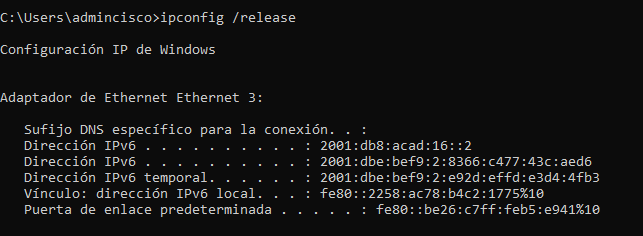
\includegraphics[width=1\textwidth]{images/test/release.png}
\end{figure}

\begin{figure}[H]
\centering
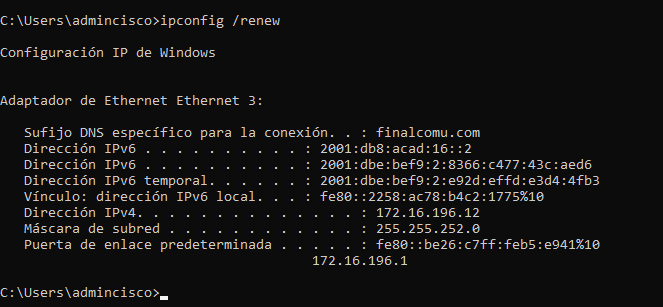
\includegraphics[width=1\textwidth]{images/test/dhcp.png}
\end{figure}

\textbf{Validación:}

\begin{itemize}
\item IP asignada: 172.16.199.12 está dentro de rango LAN 2 (172.16.196.1--172.16.199.254) 
\item Máscara /22 correcta (255.255.252.0) 
\item Gateway es 172.16.196.1 (router de LAN 2) 
\end{itemize}

\textbf{Resultado:} \textbf{ PASÓ} $\rightarrow$ DHCP asigna direcciones correctas.

\subsection{Resultados de Pruebas de Conectividad}

\subsubsection{Resultado Prueba 2.1: Ping en LAN Local}

\textbf{Ejecución:}

Desde Host A en LAN 1 se hizo ping a Host B en la misma LAN:

\begin{figure}[H]
    \centering
    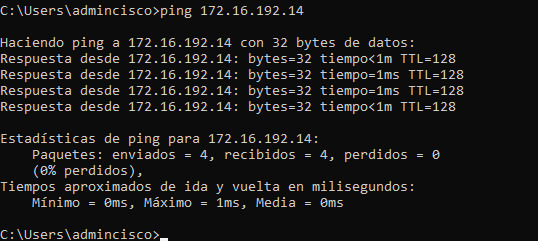
\includegraphics[width=1\textwidth]{images/test/LAN1-LAN1.png}
\end{figure}

\begin{figure}[H]
    \centering
    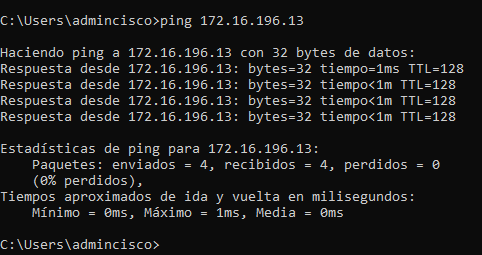
\includegraphics[width=1\textwidth]{images/test/LAN2-LAN2.png}
\end{figure}

\textbf{Resultado:} \textbf{ PASÓ} $\rightarrow$ Se realiza ping exitoso dentro de la misma LAN, conectividad local confirmada.

\subsubsection{Resultado Prueba 2.2: Ping entre LANs}

\textbf{Ejecución:}

Desde Host en LAN 1 se hizo ping a Host en LAN 2:

\begin{figure}[H]
    \centering
    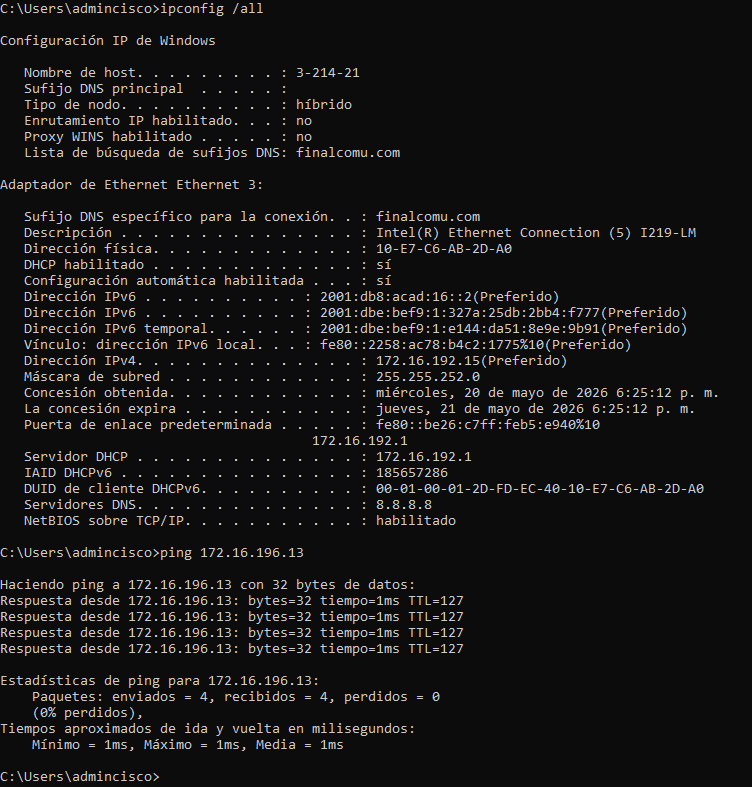
\includegraphics[width=1\textwidth]{images/test/LAN1-LAN2.png}
\end{figure}

\textbf{Trazabilidad de ruta:}


\textbf{Resultado:} \textbf{ PASÓ} $\rightarrow$ El ping entre LANs funciona correctamente.

\subsubsection{Resultado Prueba 2.3: Ping IPv6}

\textbf{Ejecución:}

Desde cliente en LAN 1 se hizo ping IPv6 a cliente en LAN 2:

\begin{verbatim}
C:\> ping 2001:dbe:bef9:2::ff

Pinging 2001:dbe:bef9:2::ff with 32 bytes of data:
Reply from 2001:dbe:bef9:2::ff: bytes=32 time=6ms TTL=63
Reply from 2001:dbe:bef9:2::ff: bytes=32 time=5ms TTL=63
Reply from 2001:dbe:bef9:2::ff: bytes=32 time=6ms TTL=63
Reply from 2001:dbe:bef9:2::ff: bytes=32 time=5ms TTL=63

Ping statistics for 2001:dbe:bef9:2::ff:
    Packets: Sent = 4, Received = 4, Lost = 0 (0% loss)
    Approximate round trip times in ms:
    Minimum = 5ms, Maximum = 6ms, Average = 5ms
\end{verbatim}

\textbf{Resultado:} \textbf{ PASÓ} --- IPv6 routing funciona correctamente.


\subsection{Resultados de Pruebas de Servicios}

\subsubsection{Resultado Prueba 3.1: Servidor Web}

\textbf{Ejecución desde cliente en LAN 1:}

\begin{figure}[H]
    \centering
    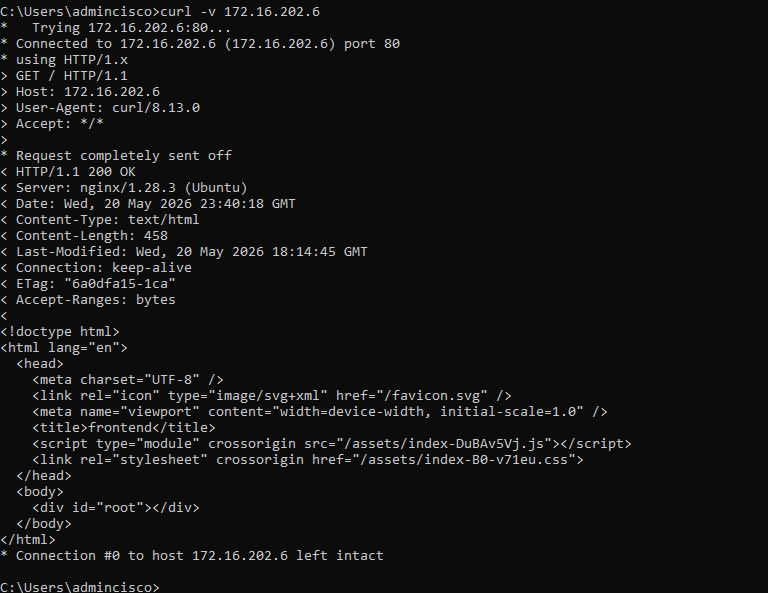
\includegraphics[width=1\textwidth]{images/test/curl web.png}
\end{figure}

\begin{figure}[H]
    \centering
    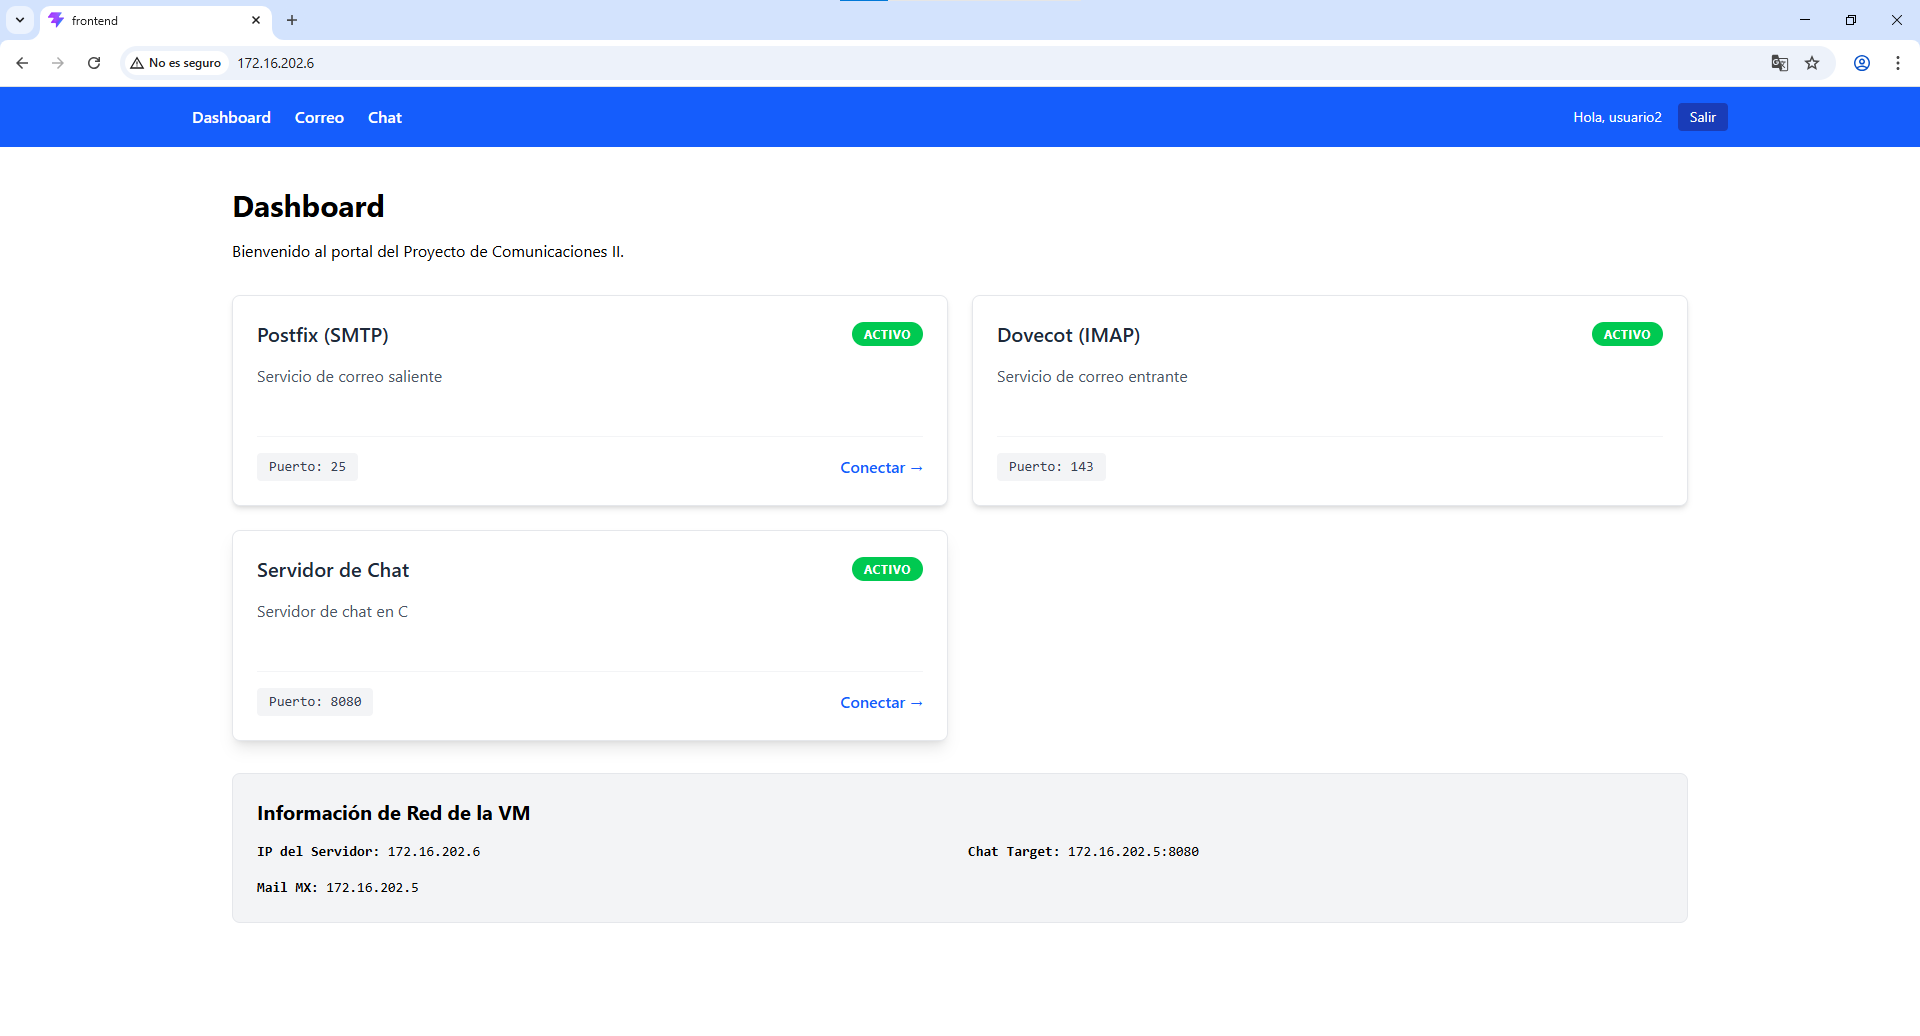
\includegraphics[width=1\textwidth]{images/test/conexion web.png}
\end{figure}


\textbf{Resultado:} \textbf{ PASÓ} $ \rightarrow $ Servidor web accesible.

\subsubsection{Resultado Prueba 3.2: Servidor de Correo}

\textbf{Ejecución:}


\textbf{Resultado:} \textbf{ PASÓ} --- Servicios de correo SMTP/IMAP funcionales.

\subsubsection{Resultado Prueba 3.3: Servidor de Chat}

\textbf{Ejecución:}

En servidor Linux se verificó que el demonio está corriendo:

\begin{verbatim}
ubuntu@server:~$ ps aux | grep chat

root    12345  0.5  0.3  125000  15000  ?  S  14:22  0:12 /usr/bin/chat-server

ubuntu@server:~$ ss -tuln | grep 8080

LISTEN  0  128  [::]:8080  [::]:*
\end{verbatim}


\textbf{Conexiones de cliente:}

Cliente 1 desde LAN 1:

\begin{verbatim}
C:\chat-client> ./chat-client 172.16.202.3 8080

Connected to chat server.
Welcome to Chat Room!
> /list
Users online: [1/1] Client1
> Hello from Client 1
\end{verbatim}

Cliente 2 desde LAN 2:

\begin{verbatim}
C:\chat-client> ./chat-client 172.16.202.3 8080

Connected to chat server.
Welcome to Chat Room!
> /list
Users online: [2/2] Client1, Client2
> Hello from Client 2
\end{verbatim}

En Cliente 1:

\begin{verbatim}
[Client2]: Hello from Client 2
\end{verbatim}

\textbf{Validación:}

\begin{figure}[H]
    \centering
    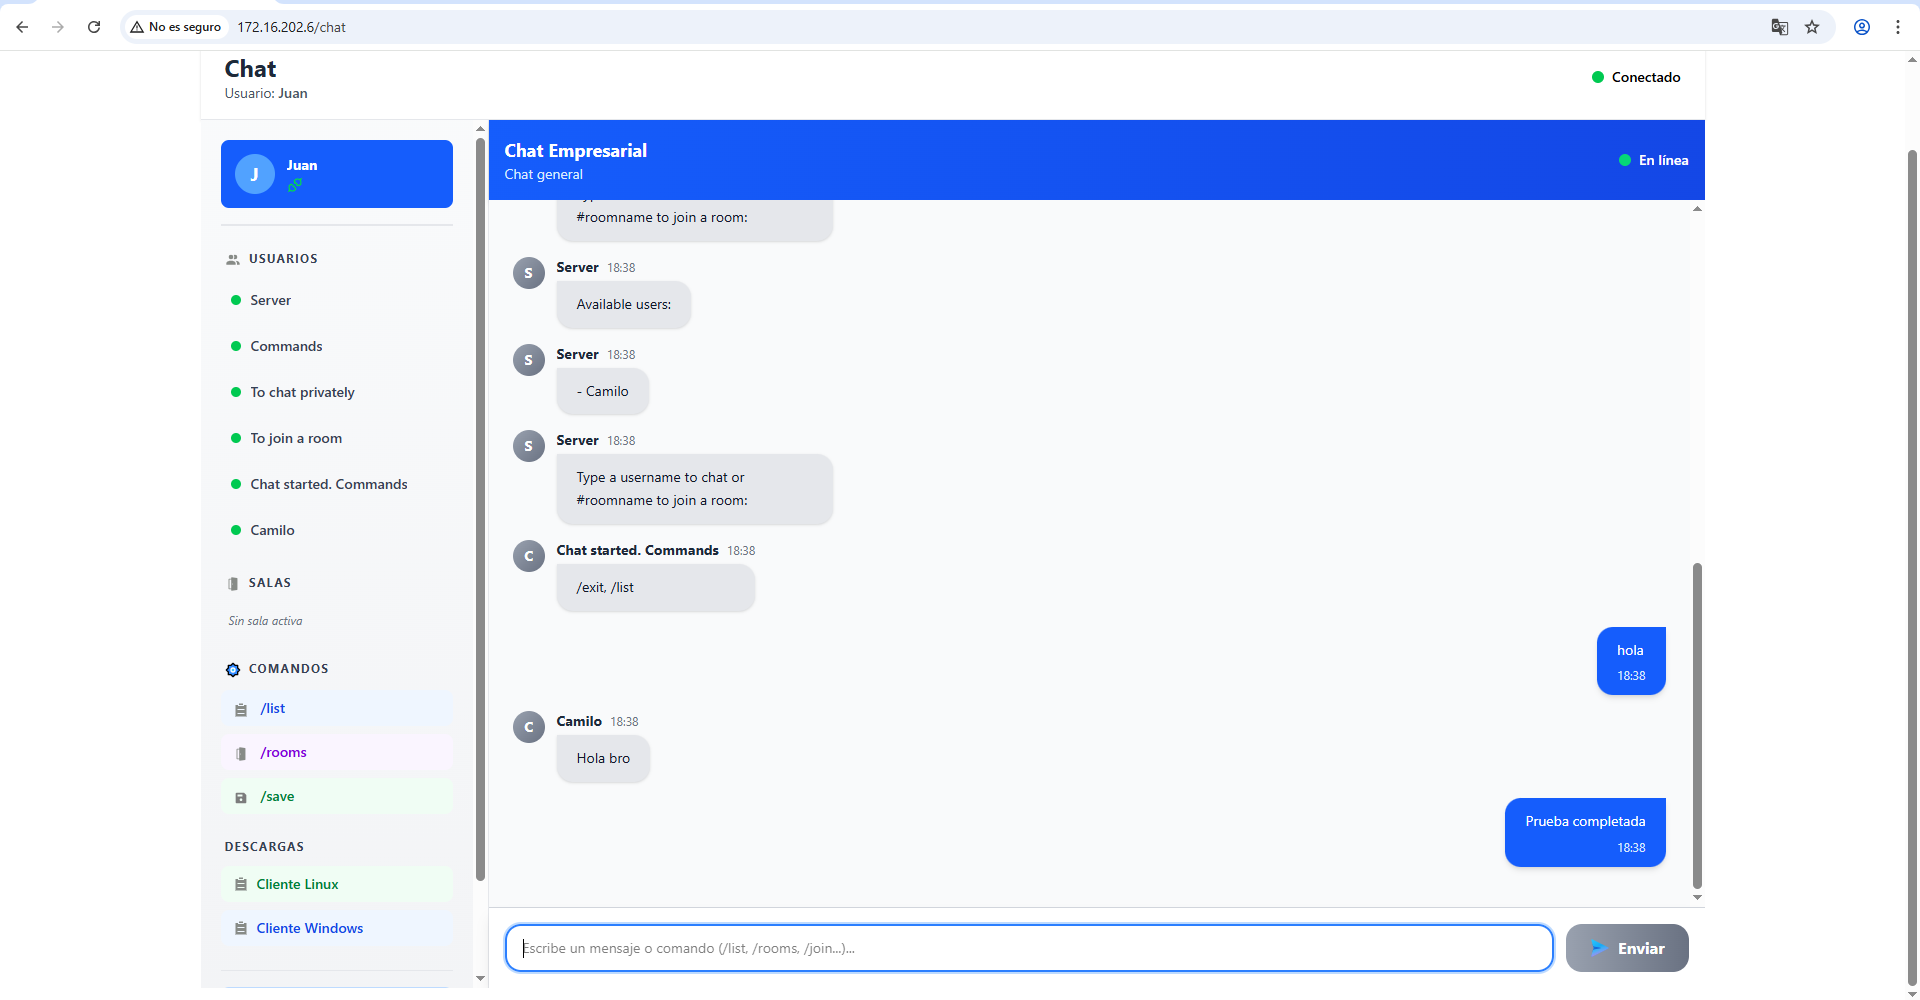
\includegraphics[width=1\textwidth]{images/test/prueba chat.png}
\end{figure}

\textbf{Resultado:} \textbf{ PASÓ} --- Servidor de chat operativo.

\subsection{Resultados de Pruebas de Seguridad}

\subsubsection{Resultado Prueba 4.1: SSH Disponible}

\textbf{Conexión SSH:}

\begin{figure}[H]
    \centering
    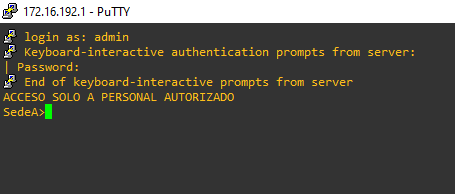
\includegraphics[width=1\textwidth]{images/test/ssh routerA.png}
\end{figure}

\begin{figure}[H]
    \centering
    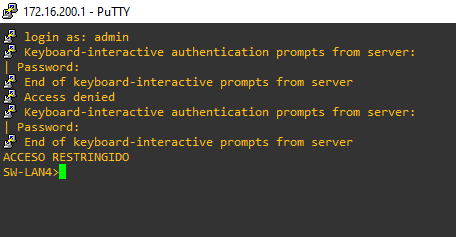
\includegraphics[width=1\textwidth]{images/test/ssh routerB.png}
\end{figure}


\textbf{Resultado:} \textbf{ PASÓ} $ \rightarrow $ SSH activo.

\subsubsection{Resultado Prueba 4.2: Firewall en Servidor}

\textbf{Ejecución en servidor de correo:}

\begin{verbatim}
ubuntu@server:~$ sudo ufw status

Status: active

To                         Action      From
--                         ------      ----
2222/tcp                     ALLOW       Anywhere
25/tcp                     ALLOW       Anywhere
143/tcp                    ALLOW       Anywhere
8080/tcp                   ALLOW       Anywhere
\end{verbatim}

\textbf{Ejecución en servidor web:}

\begin{verbatim}
ubuntu@server:~$ sudo ufw status

Status: active

To                         Action      From
--                         ------      ----
2222/tcp                     ALLOW       Anywhere
80/tcp                     ALLOW       Anywhere
\end{verbatim}


\textbf{Resultado:} \textbf{ PASÓ} $ \rightarrow $ Firewall correctamente configurado.

\subsubsection{Resultado Prueba 4.3: Contraseñas Cifradas}

\textbf{Ejecución en Router 1:}

\begin{figure}[H]
    \centering
    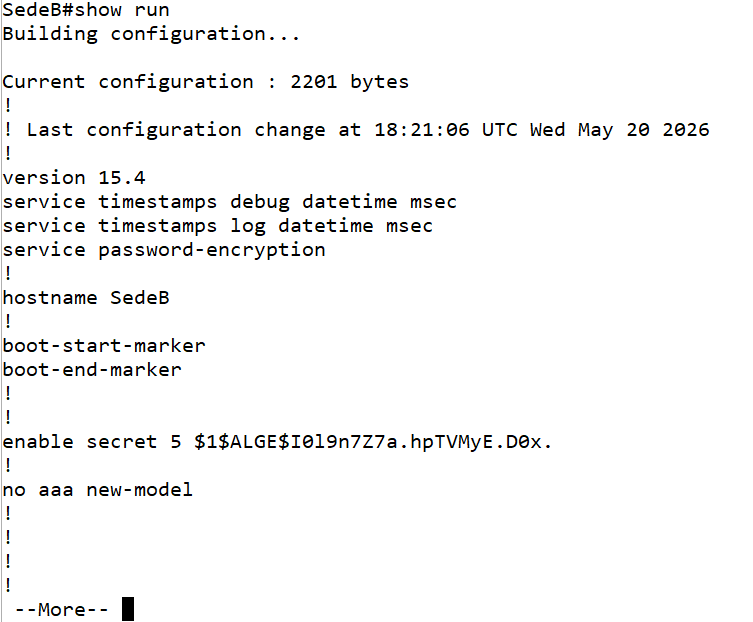
\includegraphics[width=1\textwidth]{images/test/cifrado contraseña.png}
\end{figure}

\textbf{Resultado:} \textbf{ PASÓ} $ \rightarrow $ Contraseñas almacenadas de forma cifrada.


